\scanpage{67}
\mspage{66}
% E: text|upper left|c'est qu'il semble que sur la carte
c'est qu'il semble que sur la \unsure{carte|surface} $\mathcal X$ obtenue par recollement, on n'ait aucune interprétation des ``trous'' (ou sommets, quand on a bouché les trous) en termes de la géométrie de $\underline\Sigma$.
% E: margin note|left margin beside Il faudrait|emphasis mark
\margin{\unsure{*}}
% E: text|left middle and lower|Il faudrait quand même que j'y songe
Il faudrait quand même que j'y songe, pour voir si je \unsure{ne m'étais} pas mélangé les pinceaux\ldots{} Quand on a fait ce recollement, et qu'on suit par continuité une orientation donnée $\omega$ de $\Delta_D$ (définie par une or. $\omega_D$ de $D$) en passant de $\Delta_D$ dans $\Delta_{D'}$ via l'arc de transition, on trouve \deleted{que} une orientation $\omega'$ de $\Delta_{D'}$ qui induit sur $D'$ une orientation $\omega_{D'}$ qui est \uuline{opposée} de celle déduite par transport \deleted{\unsure{de la droite}} parallèle! Voilà donc rectifiée une erreur monumentale, commise dès le début!
% E: text|upper right|Venons-en à l'autre choix
Venons-en à l'autre choix qui donne lieu à $\mathcal X\longrightarrow X$, savoir $\alpha=a$. On est obligé ici de \unsure{porter|déporter} comme j'avais dit $\Delta_D,b$ et $(\Delta_{D'},a)$, pour faire se rencontrer $b$ et $a$ dans $b^*\sim a^*\subset X$. On trouve la figure
% E: drawing|right middle|omega'=-omega delta omega_D omega_D'
\figure{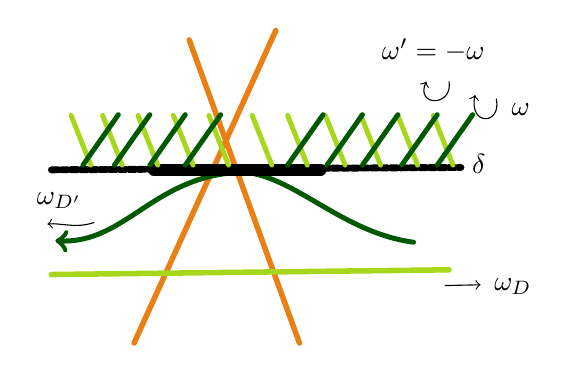
\begin{tikzpicture}[x=1cm,y=1cm,line cap=round,line join=round]
\draw[orange!65!brown,line width=2pt] (-.85,1.9)--(.55,-1.95);
\draw[orange!65!brown,line width=2pt] (.25,2.02)--(-1.55,-1.95);
\draw[green!35!black,line width=1.8pt,<-] (-2.55,-.65) .. controls (-1.65,-.7) and (-1.3,.2) .. (-.15,.22) .. controls (.5,.16) and (1.1,-.55) .. (2,-.67);
\draw[->] (-2.06,-.42)..controls (-2.3,-.5) and (-2.48,-.42)..(-2.65,-.44);
\node[above] at (-2.5,-.37) {$\omega_{D'}$};
\draw[yellow!65!green,line width=2pt] (-2.6,-1.08)--(2.45,-1.02);
\draw[->] (2.4,-1.22)--(2.85,-1.21);\node[right] at (2.9,-1.23) {$\omega_D$};
\draw[densely dotted,line width=2.5pt] (-2.6,.25)--(2.6,.28);
\draw[line width=4.2pt] (-1.3,.25)--(.82,.25);
\foreach \x in {-2.2,-1.8,-1.35,-.9,-.45,.1,.55,1.03,1.48,1.95,2.4}{\draw[yellow!65!green,line width=1.8pt] (\x-.15,.94)--(\x+.1,.31);}
\foreach \x in {-2.2,-1.8,-1.35,-.9,.4,.9,1.35,1.85,2.3}{\draw[green!35!black,line width=1.8pt] (\x,.31)--(\x+.45,.95);}
\draw[->] (2.45,1.37) .. controls (2.5,1.05) and (2.02,1.05) .. (2.16,1.37);
\node[above] at (2.25,1.5) {$\omega'=-\omega$};
\draw[->] (3.05,1.15) .. controls (3.12,.82) and (2.7,.8) .. (2.78,1.2);\node[right] at (3.12,1.02) {$\omega$};
\node[right] at (2.62,.32) {$\delta$};
\end{tikzpicture}}
% E: text|lower right|ici on recolle avec elle-même
ici on recolle avec elle-$=$ \uline{la $=$ rive} le long de la ligne critique de spécialisation $\delta$. L'identification $b^*\longrightarrow a^*$, comme variété, est l'iso. de transport. Ici la combinatoire (choix \inserted{d'objets} de structure polygonale sur l'arc de transition associé à une p.r.) est sujette au choix opéré
